\section{Objetivos}
\label{sec:objetivos}

A partir de la formulación del problema central y la metodología de planificación del Marco Lógico, se establecen los objetivos que orientan el desarrollo técnico y científico de la investigación.

\subsection{Objetivo General}
Desarrollar un sistema automatizado, basado en técnicas de Aprendizaje Automático Supervisado (\textit{Machine Learning}), que contraste el ingreso operativo declarado por medianas y grandes empresas bolivianas contra el ingreso esperado derivado de su estructura productiva real (fuerza laboral, remuneraciones salariales, materias primas, gastos de energía y activos de capital), proveyendo estimaciones cuantitativas imparciales, intervalos de predicción al 90\% y un mecanismo de priorización de riesgo para contribuir a la consistencia estadística de Cuentas Nacionales y la eficiencia fiscalizadora.

\subsection{Objetivos Específicos}
\begin{enumerate}
    \item \textbf{Diseñar e implementar un pipeline de preprocesamiento reproducible y robusto:} Automatizar la ingesta de los módulos de la encuesta EAIMCS 2017--2018, la sustitución rigurosa de valores centinela (\texttt{99999.0}), la agregación relacional a nivel de empresa de las compras y consumos de materias primas (Sección 10), y el blindaje metodológico contra fuga de información (\textit{anti-leakage}), preservando la confidencialidad establecida por el Decreto Ley N$^\circ$ 1405.
    \item \textbf{Entrenar, calibrar y comparar empíricamente modelos de regresión supervisada:} Evaluar el rendimiento predictivo de al menos siete familias de algoritmos bajo validación cruzada estratificada (5-Fold Stratified CV) sobre datos log-transformados, aplicando la técnica no paramétrica de \textit{Duan Smearing} para corregir el sesgo sistemático de retransformación en escala monetaria (Bolivianos).
    \item \textbf{Construir un sistema de auditoría y priorización de riesgo empresarial:} Cuantificar la discrepancia entre el ingreso declarado y el ingreso esperado mediante residuos estandarizados, clasificando el 100\% de las empresas en estratos de riesgo (Bajo, Medio y Alto) y desplegando un simulador predictivo interactivo con tiempos de respuesta en sub-segundo ($< 2$ segundos).
    \item \textbf{Implementar un esquema de gobernanza MLOps y monitoreo de deriva estadística (\textit{Data Drift}):} Diseñar un módulo de detección automatizada de obsolescencia del modelo fundamentado en los tests estadísticos de Kolmogorov-Smirnov y la distancia de Wasserstein de primer orden con corrección de Bonferroni, estableciendo una cadencia de reentrenamiento documentada en registros inmutables (\texttt{registry.json}).
\end{enumerate}

\subsection{a. Árbol de Objetivos}
\label{subsec:arbol_objetivos}

El \textbf{Árbol de Objetivos} presentado en la Figura \ref{fig:arbol_objetivos} constituye la transformación operativa en positivo del árbol de problemas. En él se evidencia la relación medios-fines que garantiza que cada componente y actividad técnica aporte de manera demostrable a la consecución del propósito central del proyecto y a su contribución de impacto a nivel nacional.

\begin{figure}[htbp]
\centering
\caption{Árbol de Objetivos: Medios, Componentes y Fines de Impacto del Proyecto.}
\label{fig:arbol_objetivos}
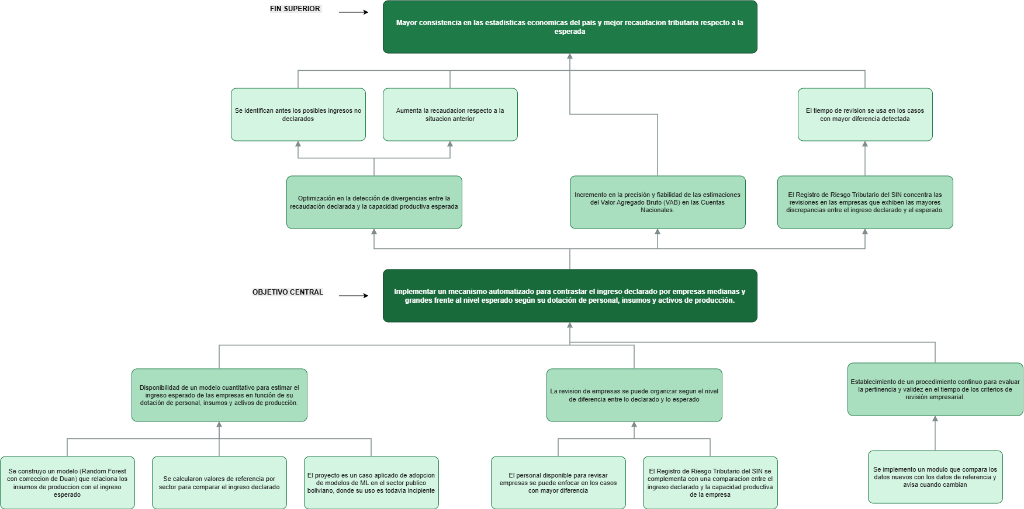
\includegraphics[width=\textwidth,keepaspectratio]{imagenes/arbol_objetivos.png}
\vspace{1mm}
\raggedright\footnotesize
\textit{Nota.} Diagrama de medios-fines derivado del árbol de problemas, estructurado para orientar los componentes del sistema hacia la consistencia fiscal y de Cuentas Nacionales.
\end{figure}

Como se esquematiza en la Figura \ref{fig:arbol_objetivos}, el \textbf{Objetivo Central} persigue \textit{implementar un mecanismo automatizado para contrastar el ingreso declarado por empresas medianas y grandes frente al nivel esperado según su dotación de personal, insumos y activos de producción}. Este propósito se materializa a través de tres ramas de medios directos y actividades:
\begin{enumerate}
    \item \textbf{Disponibilidad de un modelo cuantitativo de estimación:} Construcción de un algoritmo supervisado robusto (Random Forest calibrado con factor de corrección de Duan) que relaciona los insumos productivos con el ingreso esperado, derivando valores técnicos de referencia por macrosector económico como caso aplicado de adopción de Machine Learning en el sector público boliviano.
    \item \textbf{Focalización y priorización de la revisión empresarial:} Organización analítica de los contribuyentes en función de la magnitud de la discrepancia detectada entre lo declarado y lo estimado, permitiendo que el personal disponible concentre sus esfuerzos en los casos críticos y complementando el Registro de Riesgo Tributario del SIN con una perspectiva de capacidad productiva.
    \item \textbf{Procedimiento continuo de evaluación y vigencia:} Implementación de un módulo de monitoreo que compara las nuevas distribuciones de datos con los conjuntos de referencia históricos, emitiendo alertas tempranas ante variaciones coyunturales o estructurales (\textit{Data Drift}).
\end{enumerate}

La articulación sinérgica de estos medios converge hacia un \textbf{Fin Superior}: alcanzar una \textit{mayor consistencia en las estadísticas económicas del país y una mejor recaudación tributaria respecto a la esperada}, permitiendo identificar oportunamente ingresos no declarados, elevar la precisión del Valor Agregado Bruto (VAB) en Cuentas Nacionales y optimizar el tiempo de auditoría fiscal.
